%F-t Diagram
\documentclass[11pt,tikz,border=1]{standalone}
\usepackage{xcolor}
\definecolor{r1}{HTML}{FF8674}
\definecolor{b1}{HTML}{17ABDD}
\definecolor{p1}{HTML}{D4B6D6}
\definecolor{g1}{HTML}{70E2CB}
\usepackage{mathptmx}

\begin{document}
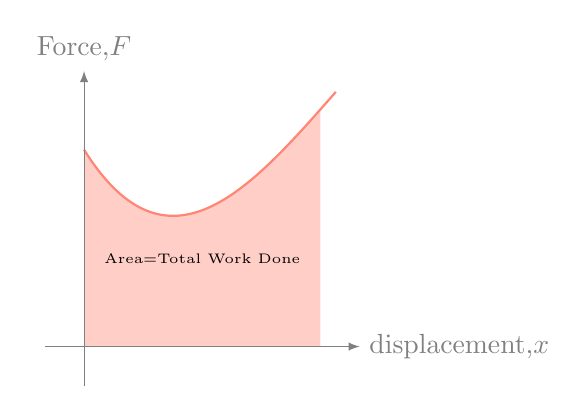
\begin{tikzpicture}
  	\fill [fill=r1!40!white, domain=0:3, variable=\x] (0, 0) -- plot ( {\x}, {-0.09*\x^3+0.86*\x^2-1.6*\x+2.5}) -- (3, 0) -- cycle; %填充函数的表达式。从左侧最低点开始,然后到函数曲线,再到右侧断电,--cycle形成封闭面积。
  	\draw [color=r1,thick,domain=0:3.2,samples=200] plot (\x,-0.09*\x^3+0.86*\x^2-1.6*\x+2.5); 
  	\draw [-latex,gray] (-.5,0)--(3.5,0) node[right] {displacement,$x$};
	\draw [-latex,gray] (0,-0.5)--(0,3.5) node[above] {Force,$F$};
	\node at (1.5,1.3)[below] {\tiny{Area=Total Work Done}};
\end{tikzpicture}
\end{document}